\begin{frame}{Hybrid rocket engine structure}
  \centering
  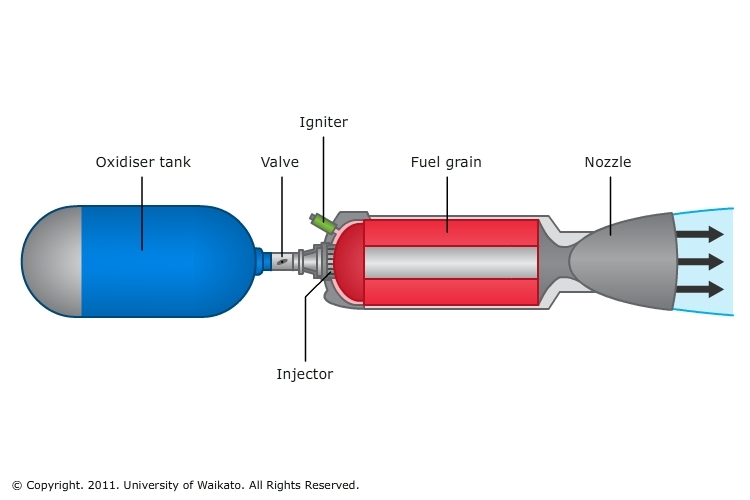
\includegraphics[width=\columnwidth]{figures/Hybrid-rocket-engine.jpg}
\end{frame}

\begin{frame}{Calculations program requirements}
  \begin{itemize}
  \item[--] \emph{Readable:} more than one person needs to be able to understand
    it
  \item[--] \emph{Extensible:} working groups should be able to extend their
    parts without impacting the rest of the assembly
  \item[--] \emph{General:} not committing to a particular design
  \end{itemize}
\end{frame}

\begin{frame}{OpenMDAO framework}
  \center{
    Solution: \textbf{OpenMDAO!}

    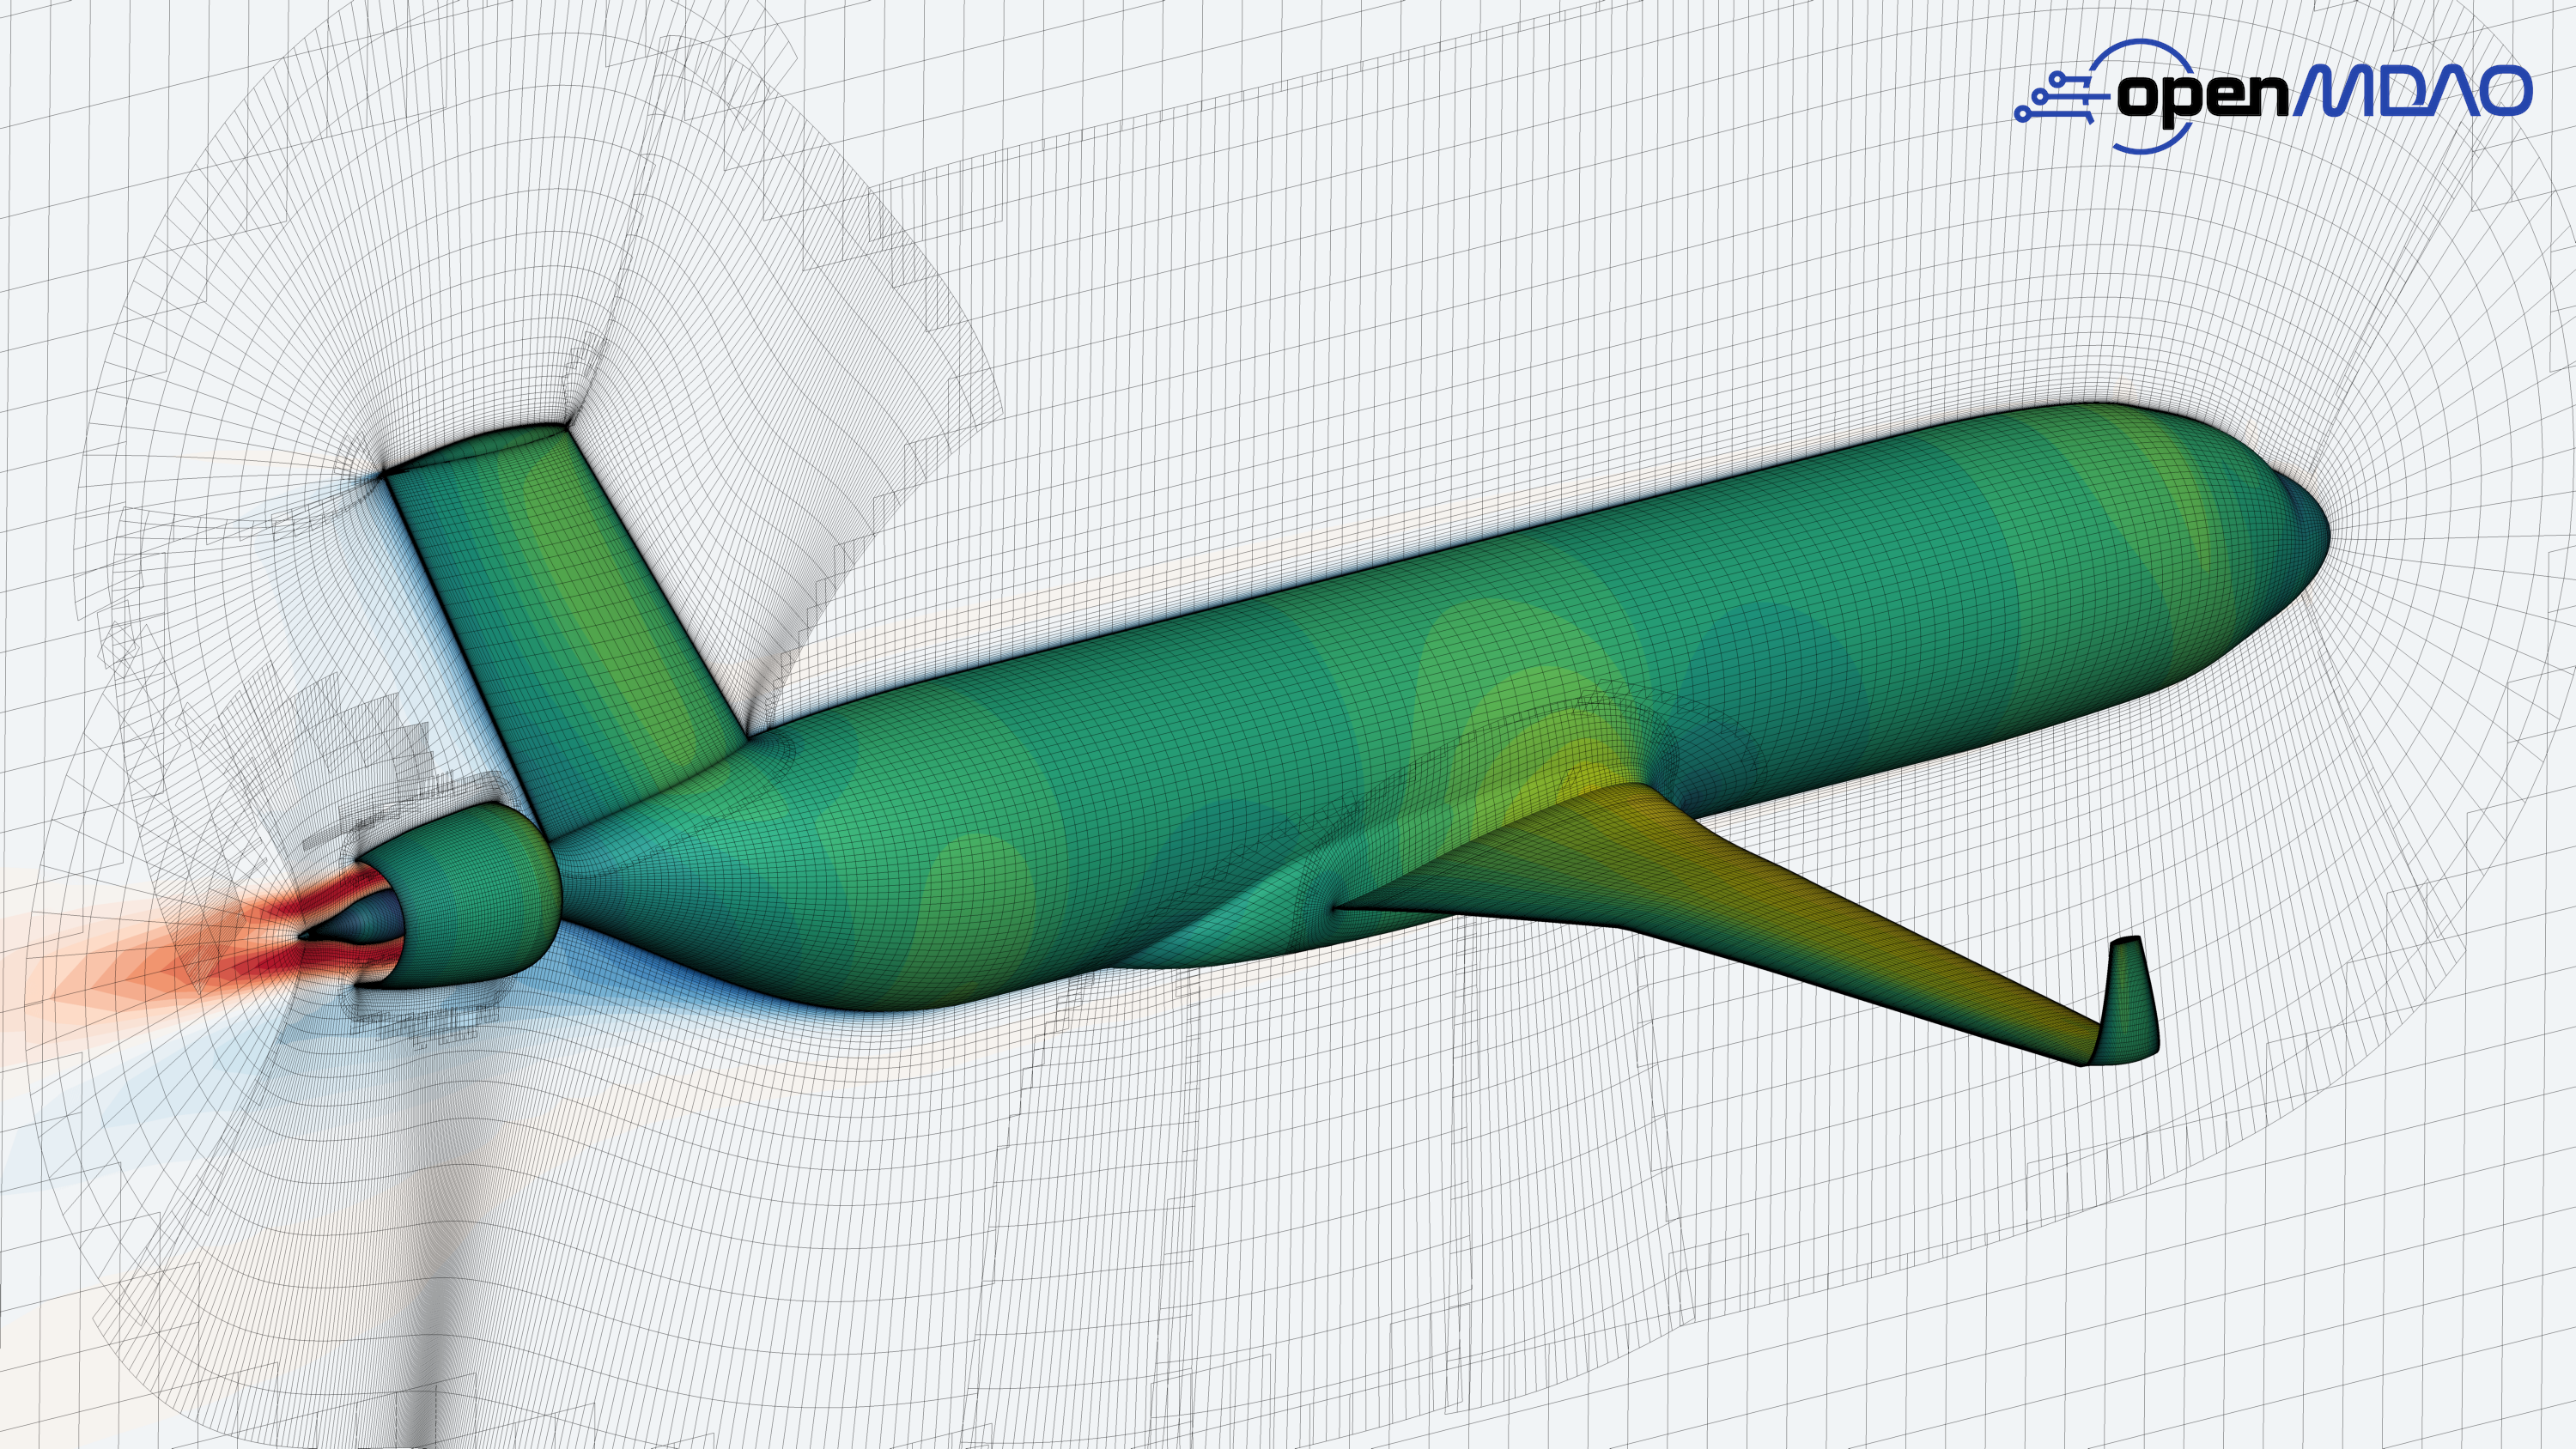
\includegraphics[
      width=0.8\columnwidth
    ]{figures/openmdao_slide.png}
  }

  (Multi-Disciplinary Analysis and Optimization)

  \vspace{\baselineskip}

  \begin{itemize}
  \item[--] Python OOP
  \item[--] Industry standard
  \end{itemize}
\end{frame}

\begin{frame}{OpenMDAO class structure}
  \center{
    \phantom{(These are the parts we care about)}
    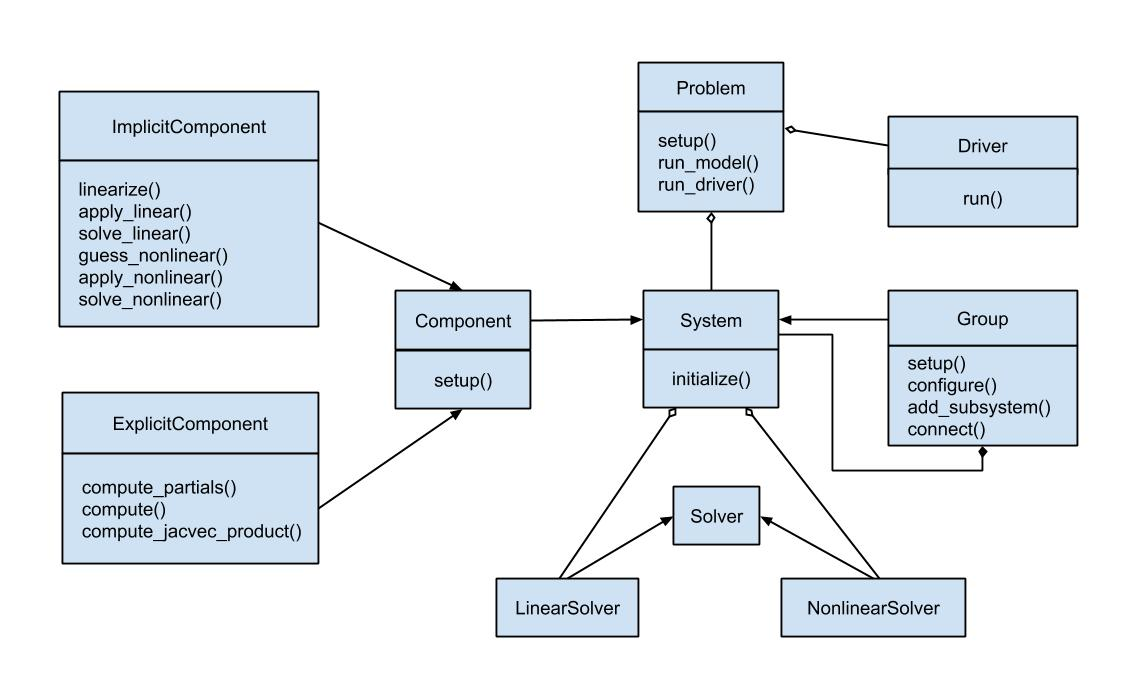
\includegraphics[
      width=\columnwidth
    ]{figures/openmdao_class_structure.jpg}
  }
\end{frame}

\begin{frame}{OpenMDAO class structure}
  (These are the parts we care about)

  \center{
    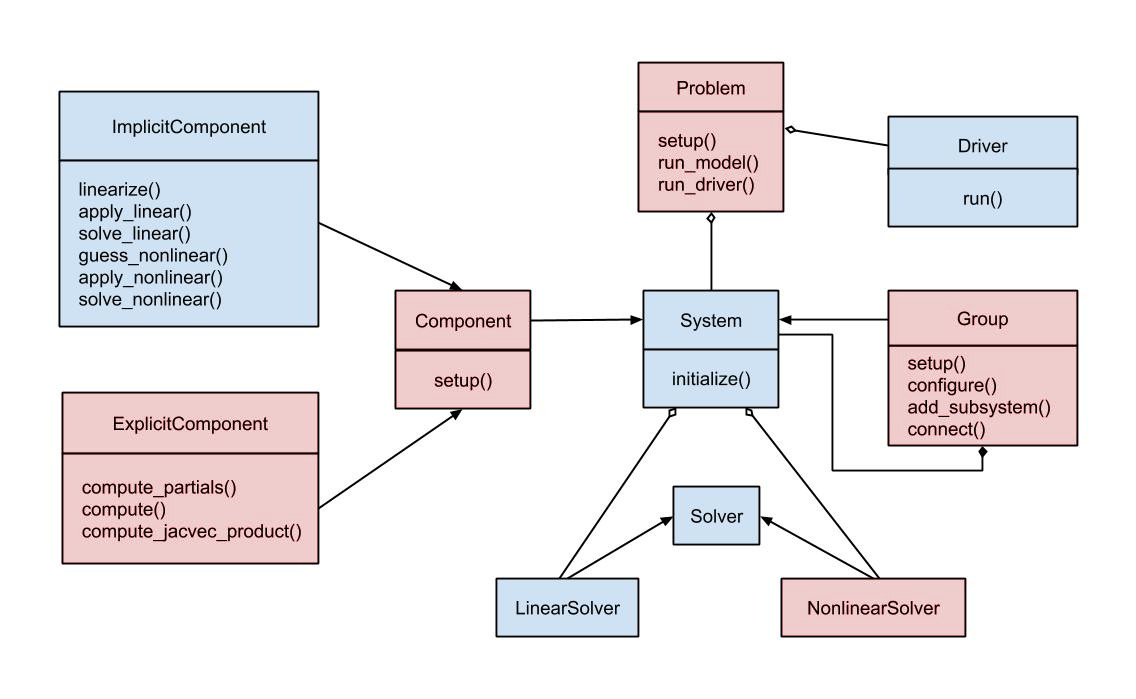
\includegraphics[
      width=\columnwidth
    ]{figures/openmdao_class_structure_highlight.jpg}
  }
\end{frame}

\begin{frame}{OpenMDAO class structure}
  This assembles into a tree-like structure with

  \begin{itemize}
  \item[--] \lstinline{Problem}'s internal Model class at root,
  \item[--] \lstinline{Group} intances as branching nodes, and
  \item[--] \lstinline{Component} instances as leaves:
  \end{itemize}

  \vspace{\baselineskip}

  \center{
    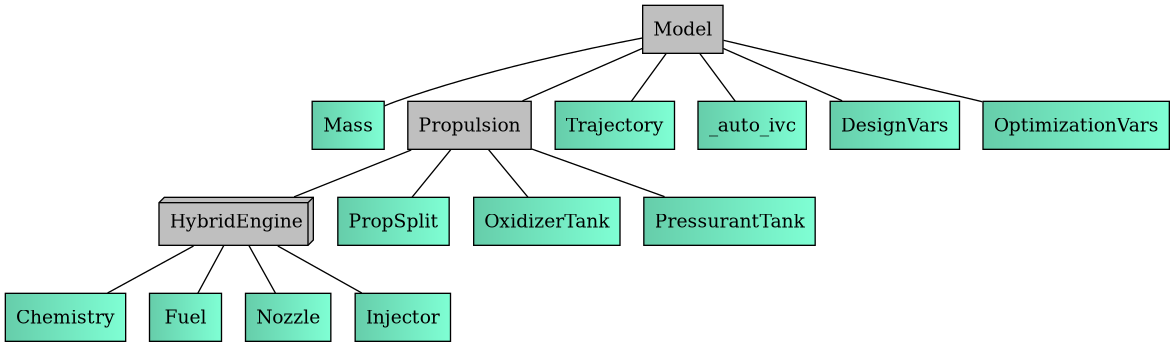
\includegraphics[width=\columnwidth]{figures/rocket_tree.png}
  }
\end{frame}

\begin{frame}{OpenMDAO class structure}
  \emph{Readability:} What does the code for this look like?

  \pause
  \vspace{\baselineskip}

  In the following: \emph{OpenMDAO by example}
\end{frame}
